\documentclass[10pt]{article}
\usepackage[utf8]{inputenc}
\usepackage[doublespacing]{setspace}
\usepackage{textcomp}
\usepackage{amsmath,amssymb,amsthm}
\usepackage{fancyhdr}
\usepackage{lastpage}
\usepackage[]{hyperref}
\usepackage[pdftex]{graphicx}
\usepackage{ctex}
\usepackage{booktabs}
\usepackage{subfigure}
\usepackage{titlesec}
\usepackage{listings}
\usepackage{enumerate}
\usepackage{bm}
\usepackage{float}
%\allowdisplaybreaks
\renewcommand{\contentsname}{\centerline{Contents}}
\pagestyle{fancy}
\author{D}
\def\name{D}
\lhead{Time Series Methods}
\chead{}
\rhead{\name}
\cfoot{-\space\thepage\space-}
\newtheorem{exer}{\bm{$Exercise$}}
\newtheorem{prob}{\bm{$Problem$}}
\newtheorem{bonus}{\bm{$Bonus\;Problem$}}
\newcommand{\tabincell}[2]{\begin{tabular}{@{}#1@{}}#2\end{tabular}}
\CTEXoptions[today=old]

\begin{document}

\title{Assignment Two}
\date{\today}
\maketitle
\thispagestyle{fancy}
\thispagestyle{fancy}

\begin{prob}
\end{prob}
\begin{enumerate}[1)]
\vspace{3mm}

\item
A time series is weakly stationary when
\subitem
a) all observations have the same finite variance;
\subitem
b) all observations have the same mean;
\subitem
c) the covariance of the observations at any two time points depends only on the difference in time between the two time points.
\vspace{3mm}

\item
The two differences between weak and strict stationarity are that
\subitem
a) strict stationarity requires that all observations have the same distribution while weak stationarity does not;
\subitem
b) strict stationarity requires that the shifted values have the same distribution as the original observations while weak stationarity does not. % Comment: same
\vspace{3mm}

\item
We have
\begin{align*}
\gamma_X(h)=\left\{\begin{array}{ll}COV[X_{t+h},X_t]=\mathbb{E}[(X_{t+h}-\mu_X)(X_t-\mu_X)],\;\textrm{if}\;h\geq0;\\
\gamma_X(-h),\;\textrm{if}\;h<0.\end{array}\right.
\end{align*}
The estimator of the autocovariance function of a stationary time series is
\begin{align*}
\hat{\gamma}_x(h)=\left\{\begin{array}{ll}\frac{1}{n}\sum^{n-h}_{t=1}(x_{t+h}-\hat{\mu}_x)(x_t-\hat{\mu}_x),\;\textrm{if}\;h\geq0;\\
\hat{\gamma}_x(-h),\;\textrm{if}\;h<0.\end{array}\right.
\end{align*}
\vspace{3mm}

\item
We have
\begin{align*}
\rho_X(h)=\frac{\gamma_X(h)}{\gamma_X(0)}.
\end{align*}
The estimator of the autocorrelation function of a stationary time series is
\begin{align*}
\hat{\rho}_X(h)&=\frac{\hat{\gamma}_X(h)}{\hat{\gamma}_X(0)}\\
&=\frac{\sum^{n-|h|}_{t=1}(X_{t+|h|}-\hat{\mu}_X)(X_t-\hat{\mu}_X)}{\sum^{n}_{t=1}(X_t-\hat{\mu}_X)(X_t-\hat{\mu}_X)}
\end{align*}

\end{enumerate}
\vspace{3mm}

\begin{prob}
\end{prob}
\begin{enumerate}[1)]
\vspace{3mm}

\item
Yes, I will assume this time series is stationary, since approximately its probabilistic behavior does not change as the time series is shifted in time. All observations have similar means and variances. The type of this stationarity may be ``deep sleep''. % Comment: ?
\vspace{3mm}

\item
No, I will not assume this time series is stationary, since the upward trend is significant and the fluctuation increases. Both the means and variances roughly increase as time goes.
\vspace{3mm}

\item
No, I will not assume this time series is stationary, since its variance is not finite for
\begin{align*}
VAR[X_t]=\mathbb{E}[X^2_t]-\mu^2=\frac{\sigma^2_W}{1-1}=\infty. % Comment: ?
\end{align*}
\vspace{3mm}

\item % Comment: do not need to 'assume' for theoretical t.s.; we know if they are / aren't!
Yes, I will assume this time series is stationary, since all moving average time series are stationary.\footnote{ Wikipedia contributors. (2019). Moving-average model. \textit{Wikipedia}. Retrieved from https://en.wikipedia.org/w/index.php?title=Moving-average\_model\&oldid=911245323/.} Specifically for this MA(1) series, all observations have the same mean 0, the same finite variance
\begin{align*}
VAR[W_t+0.7W_{t-1}]=VAR[W_t]+0.49VAR[W_{t-1}]=1.49\sigma^2_W
\end{align*}
and the covariance is independent of t for
\begin{align*}
\gamma_X(h)=\gamma_X(t+h,t)=\left\{\begin{array}{ll}1.49\sigma^2_W,\;\textrm{if}\;h=0;\\
0.7\sigma^2_W,\;\textrm{if}\;h=1;\\
0,\;\textrm{if}\;h>1.\end{array}\right.
\end{align*}

\end{enumerate}
\vspace{3mm}

\begin{prob}
\end{prob}
\begin{enumerate}[1)]
\vspace{3mm}

\item
The mean is 6.003731.\\
R codes:
\lstinputlisting{p31a.R}
\vspace{3mm}

\item
R codes:
\lstinputlisting{p32a.R}
R outputs:\\
Autocovariances of series `unemp', by lag
\lstinputlisting{p32a.txt}
\begin{figure}[H]
  \centering
  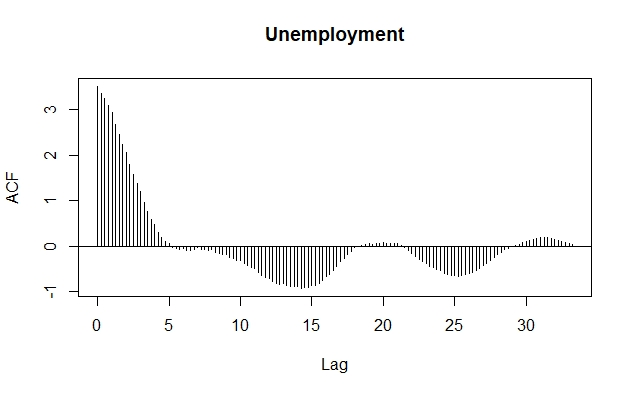
\includegraphics[width=8cm,height=5cm]{p32a.jpeg}
  \caption{Sample Autocovariance Function}
\end{figure}
\vspace{3mm}

\item
R codes:
\lstinputlisting{p33a.R}
R outputs:\\
Autocorrelations of series `unemp', by lag
\lstinputlisting{p33a.txt}
\begin{figure}[H]
  \centering
  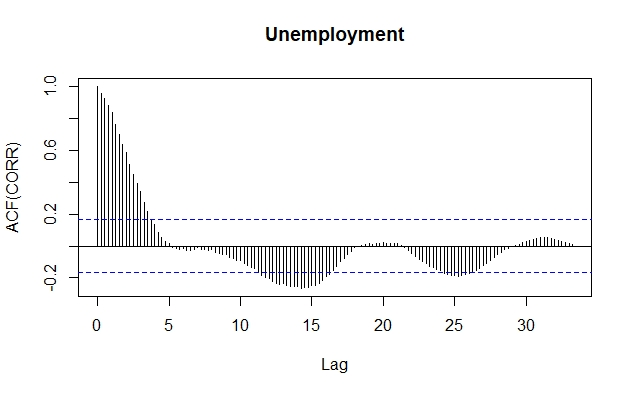
\includegraphics[width=8cm,height=5cm]{p33a.jpeg}
  \caption{Sample Autocorrelation Function}
\end{figure}
\vspace{3mm}

\item
The lag means how many time points are observed before the corresponding observations.\\
The height of each spike shows the value of the autocorrelation function for the lag. The large the lag is, the closer to 0 the autocorrelation value is. The value close to 0 is evidence against autocorrelation.\\
Specifically, when the lag is between 0 and 4 approximately, the employment rate is highly positively correlated to each other, meaning that if the employment rate increases it continues increasing; when the lag is between 12 and 16 approximately and at around 25, the employment rate is highly negatively correlated to each other, meaning that if the previous employment rate increases it tends to decrease.\footnote{ Anderson, A., \& Semmelroth, D. (n.d.). \textit{Autocorrelation plots: graphical technique for statistical data}. Retrieved from https://www.dummies.com/programming/big-data/data-science/autocorrelation-plots-graphical-technique-for-statistical-data/.} % Comment: "if previous rate is high, the next is likely to be high"

\end{enumerate}
\vspace{3mm}

\begin{prob}
\end{prob}
\begin{enumerate}[1)]
\vspace{3mm}

\item
R codes:
\lstinputlisting{p41a.R}
\begin{figure}[H]
  \centering
  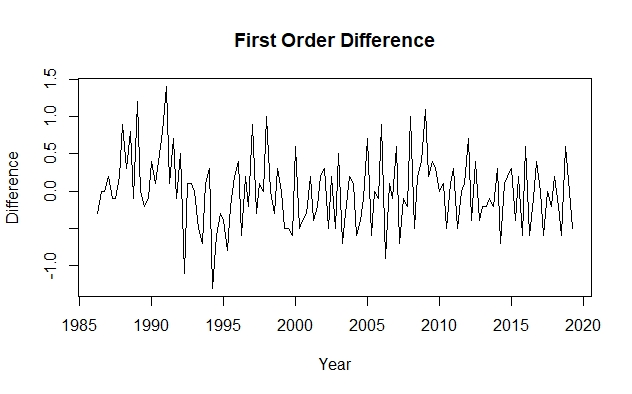
\includegraphics[width=8cm,height=5cm]{p41a.jpeg}
  \caption{Series of First Order Difference}
\end{figure}
Yes, I assume this series could be white noise, despite the fluctuation in the early stages. (Results in the later parts of this problem may suggest my assumption is wrong.) % Comment: why?
\vspace{3mm}

\item
R codes:
\lstinputlisting{p42a.R}
R outputs:\\
Box-Pierce test\\
data: diff1\\
X-squared = 4.8277, df = 3, p-value = 0.1849\\
The outputs give the value of the statistic Q and the p-value. The p-value in this case is larger than 0.05, meaning that the test gives no evidence that the series is not white noise.
\vspace{3mm}

\item
R codes:
\lstinputlisting{p43a.R}
R outputs:\\
Box-Pierce test\\
data: diff1\\
X-squared = 149.25, df = 20, p-value $<$ 2.2e-16\\
The p-value in this case is smaller than 0.05, meaning that the test gives evidence that the series is not white noise. The command above was repeated for 10 times and no false rejection showed up.
\vspace{3mm}

\item
``When too many lags are included, the test can lose power and become unreliable. Unfortunately, there is no good rule to pick the largest lag k for the test. A simple rule of thumb says that k should not be larger than n/5.''\footnote{ Lab 5 solutions. (2019). Unpublished manuscript.} Since the observations are 134 and 134/5 is 26.8 as the assumed maximum amount of lags, the result in (3) with 20 lags works well ($3<20<26.8$) and is reliable.

\end{enumerate}
\vspace{3mm}

\begin{bonus}
\end{bonus}
\begin{enumerate}[1)]
\vspace{3mm}

\item
\begin{proof}
Using the stationarity of $X_t$, we have
\begin{equation}
VAR[X_t]=VAR[X_{t-1}];
\end{equation}
\begin{equation}
COV[X_t,W_{t+|h|}]=COV[X_{t-1},W_t]=COV[\phi_1X_{t-1},W_t]=0. % Comment: ?
\end{equation}
Hence, with equations (1) and (2), we have
\begin{align*}
VAR[X_t]&=VAR[\phi_0+\phi_1X_{t-1}+W_t]\\
&=VAR[\phi_1X_{t-1}+W_t]\\
&=VAR[\phi_1X_{t-1}]+VAR[W_t]+2COV[\phi_1X_{t-1},W_t]\\
&=\phi^2_1VAR[X_{t-1}]+\sigma^2_W\\
&=\phi^2_1VAR[X_t]+\sigma^2_W\\
&=\frac{\sigma^2_W}{1-\phi^2_1}.
\end{align*}
\end{proof}
\vspace{3mm}

\item
\begin{proof}
Use the previous result,
\begin{equation}
VAR[X_t]=\frac{\sigma^2_W}{1-\phi^2_1}.
\end{equation}
With equations (2) and (3), we have
\begin{align*}
\gamma_X(h)&=COV[X_{t+h},X_t]\\
&=COV[\phi^{|h|}_1X_t+\phi^{|h|-1}_1W_{t+h}+c(\phi_0,\phi_1),X_t]\\
&=COV[\phi^{|h|}_1X_t+\phi^{|h|-1}_1W_{t+h},X_t]\\
&=\phi^{|h|}_1COV[X_t,X_t]+\phi^{|h|-1}_1COV[W_{t+h},X_t]\\
&=\phi^{|h|}_1VAR[X_t]+0\\
&=\phi^{|h|}_1\frac{\sigma^2_W}{1-\phi^2_1}.
\end{align*}
\end{proof}

\end{enumerate}

\end{document}
